\documentclass[conference]{IEEEtran}
\IEEEoverridecommandlockouts
\renewcommand{\thesection}{\Roman{section}}
\usepackage{booktabs}
\usepackage{fancyhdr}
\usepackage{algorithm}
\usepackage[usenames, dvipsnames]{xcolor}
\usepackage{algorithmic}
\usepackage{colortbl}
\usepackage{caption}
\usepackage{graphicx}
\usepackage{array}
\usepackage{adjustbox}
\usepackage{hyperref,graphicx,color,float}
\bibliographystyle{unsrt}
\definecolor{myblue}{RGB}{10, 150, 200}

\usepackage{cite}
\usepackage{multirow}
\usepackage{amsmath,amssymb,amsfonts}
\usepackage{algorithmic}
\usepackage{graphicx}
\usepackage{textcomp}
\usepackage{comment}
\definecolor{highlightColor}{HTML}{E6FFE6}

\usepackage{xcolor}
\def\BibTeX{{\rm B\kern-.05em{\sc i\kern-.025em b}\kern-.08em
    T\kern-.1667em\lower.7ex\hbox{E}\kern-.125emX}}
    
\fancypagestyle{firstpage}{
  \fancyhf{} % Clear all header and footer fields
  \renewcommand{\headrulewidth}{0pt} % Remove the header rule
  \renewcommand{\footrulewidth}{0pt} % Remove the footer rule
}

\pagestyle{empty} % Apply empty style to other pages

\makeatletter
\newcommand{\linebreakand}{%
  \end{@IEEEauthorhalign}%
  \hfill\mbox{}\par%
  \noindent\mbox{}\hfill\begin{@IEEEauthorhalign}%
}
\makeatother

\title{Multi-Method Explainability for YOLO26-Based Caries Detection in Intra-oral Photos}

\author{%
\IEEEauthorblockN{First Author Name}%
\IEEEauthorblockA{\textit{Department Name} \\%
\textit{Institution Name}\\%
City, Country \\%
author1@example.com}%
\and%
\IEEEauthorblockN{Second Author Name}%
\IEEEauthorblockA{\textit{Department Name} \\%
\textit{Institution Name}\\%
City, Country \\%
author2@example.com}%
\and%
\IEEEauthorblockN{Third Author Name}%
\IEEEauthorblockA{\textit{Department Name} \\%
\textit{Institution Name}\\%
City, Country \\%
author3@example.com}%
\linebreakand%
\IEEEauthorblockN{Fourth Author Name}%
\IEEEauthorblockA{\textit{Department Name} \\%
\textit{Institution Name}\\%
City, Country \\%
author4@example.com}%
\and%
\IEEEauthorblockN{Fifth Author Name}%
\IEEEauthorblockA{\textit{Department Name} \\%
\textit{Institution Name}\\%
City, Country \\%
author5@example.com}%
\and%
\IEEEauthorblockN{Sixth Author Name}%
\IEEEauthorblockA{\textit{Department Name} \\%
\textit{Institution Name}\\%
City, Country \\%
author6@example.com}%
}

\begin{document}
\maketitle
\thispagestyle{firstpage} % Apply the footer only on the first page

\begin{abstract}
A dentist looking at an AI-flagged caries lesion has two reasonable questions: is the model right, and why does it think so? Most segmentation models that could answer the first question well are too heavy to run chairside and too opaque to answer the second one at all. We tackle both problems with a single pipeline built on YOLO26, trained to segment nine tooth pathology classes in intra-oral photographs from the AlphaDent dataset. Against a YOLOv8x baseline evaluated at 640 px and 960 px, we test five configurations: YOLO26m and YOLO26l at both 640 px and 960 px, and YOLO26x at 960 px. The medium model turns out to be a remarkably good bargain. At its best checkpoint it reaches 0.4455 Mask mAP@50 (0.4658 Box) with 23.5M parameters and 121.2 GFLOPs, surpassing the 71.8M-parameter baseline's published 0.436 while cutting compute by 64.8\%. At 960 px, YOLO26l stretches the margin to 0.4582 Mask mAP@50, while the largest YOLO26x trails both, a reminder that model capacity should be matched to dataset size. Under the dataset authors' merged four-class protocol, YOLO26l reaches 0.6913 Mask mAP@50, surpassing the published 0.680 baseline. Training scales across GPUs through Distributed Data Parallel (roughly 1.85$\times$ faster on two Tesla T4s), and a self-healing validation routine survives the CUDA out-of-memory crashes that high-resolution dental photographs otherwise cause. To answer the ``why'' question, our YOLOExplainer module hooks into intermediate YOLO26 layers and produces class activation maps with seven attribution methods, letting clinicians see, and cross-check, exactly which image regions drive each prediction. A causal deletion/insertion evaluation across all seven methods and five configurations identifies the gradient-free Eigen-CAM as the most faithful attribution for this task, while inter-method agreement, though a useful stability summary, is found not to track prediction correctness.
\end{abstract}

\begin{IEEEkeywords}
Dental caries detection, YOLO26, instance segmentation, explainable AI, class activation mapping, distributed data parallel, intra-oral photography
\end{IEEEkeywords}

\section{Introduction}
Dental caries is among the most common chronic diseases in the world, and much of its damage is preventable if lesions are caught early. Intra-oral photography is an appealing screening channel for exactly this reason: it is cheap, radiation-free, and increasingly available even outside specialist clinics. Deep detectors have already shown they can pull clinically useful signal from dental images, from tooth detection and numbering in panoramic radiographs~\cite{tuzoff2019tooth} to interproximal caries in bitewings~\cite{bayati2025advanced}, pulp involvement in primary molars~\cite{sohrabi2025deep}, and GV Black caries classification~\cite{agulan2024detection}.

Yet two practical obstacles keep these models out of everyday practice. The first is cost: the best instance segmentation models are large, and a 70M-parameter network is a poor fit for a chairside tablet or an edge device in a rural clinic. The second is trust. A dentist cannot act on a prediction they cannot inspect, and the medical AI literature has been blunt about the need for explainability and causability before clinical adoption~\cite{holzinger2019causability, adadi2018peeking}.

We address both obstacles together. Starting from the reference YOLOv8 pipeline~\cite{jocher2023ultralytics} for the AlphaDent dataset~\cite{sosnin2025alphadent}, a collection of intra-oral photographs annotated with nine tooth pathology classes, we migrate to the YOLO26 family of unified real-time vision models~\cite{jocher2026yolo26}, whose \texttt{Segment26} head is well suited to fine-grained multi-class medical instance segmentation. Along the way we fix several engineering problems that quietly break reproducibility, and we add an explainability layer designed for clinical inspection rather than as an afterthought. Our contributions are:

\begin{itemize}
\item A YOLO26-based instance segmentation pipeline for nine-class dental pathology detection in intra-oral photographs, evaluated in five configurations (YOLO26m and YOLO26l at 640 px and 960 px, YOLO26x at 960 px) against YOLOv8x baselines at 640 px and 960 px.
\item Dynamic multi-GPU training via PyTorch Distributed Data Parallel (DDP), replacing the baseline's hard-coded single device, together with a self-healing validation routine that survives CUDA out-of-memory (OOM) events on very high-resolution images.
\item \textit{YOLOExplainer}, a self-contained module that produces class activation maps for YOLO26 predictions using seven complementary post-hoc methods, so that clinicians can visually audit which regions drive each pathology call, together with a quantitative causal-faithfulness and inter-method-agreement analysis of all seven methods.
\item An accuracy--efficiency analysis showing that YOLO26m-seg surpasses the YOLOv8x-seg baseline at roughly one third of the parameters and 35.2\% of the compute.
\end{itemize}

\section{Literature Review}
\textbf{Real-time detection and instance segmentation.} Since the original YOLO reframed detection as a single-pass regression problem~\cite{redmon2016yolo}, the family has iterated quickly: YOLOv8~\cite{jocher2023ultralytics}, YOLOv9 with programmable gradient information~\cite{wang2024yolov9}, the NMS-free end-to-end YOLOv10~\cite{wang2024yolov10}, YOLO11~\cite{ultralytics2024yolo11}, the attention-centric YOLOv12~\cite{tian2025yolov12}, and most recently YOLO26, which unifies detection, segmentation, pose, and classification in one end-to-end design~\cite{jocher2026yolo26}. On the segmentation side, Mask R-CNN~\cite{he2017maskrcnn} set the two-stage standard, while YOLACT~\cite{bolya2019yolact} showed that prototype masks could deliver real-time instance segmentation, the idea modern YOLO segmentation heads still build on.

\textbf{Deep learning in dental imaging.} Convolutional networks reached expert-level tooth detection and numbering on panoramic radiographs years ago~\cite{tuzoff2019tooth}, and recent YOLOv8 studies have moved into genuinely clinical territory: interproximal caries in bitewings~\cite{bayati2025advanced}, pulp involvement in primary molars~\cite{sohrabi2025deep}, and caries classification~\cite{agulan2024detection}. Progress, however, is bottlenecked by data. Uribe et al.\ survey the public dental dataset landscape and find it thin~\cite{uribe2024public}. AlphaDent~\cite{sosnin2025alphadent} helps by contributing densely annotated intra-oral photographs across nine pathology classes, and open frameworks such as SegmentAnyTooth target tooth enumeration and segmentation on the same modality~\cite{nguyen2025segmentanytooth}.

\textbf{Explainable AI for medical detection.} Class activation mapping began with CAM~\cite{zhou2016cam} and has since branched into a family of methods with different strengths: Grad-CAM's gradient weighting~\cite{selvaraju2017grad}, Grad-CAM++'s second-order refinement for multiple instances~\cite{chattopadhay2018grad}, the axiom-grounded XGrad-CAM~\cite{fu2020axiom}, HiRes-CAM's faithfulness guarantee~\cite{draelos2020use}, Layer-CAM's use of intermediate layers~\cite{jiang2021layercam}, and the gradient-free Eigen-CAM~\cite{muhammad2020eigen}. Post-hoc CAM analysis has been applied to YOLO-based medical diagnosis before~\cite{borah2024comprehensive}, but existing wrappers rarely speak to modern YOLO segmentation heads. Closing that gap for \texttt{Segment26} is one of the goals of this work.

\section{Methodology}
Fig.~\ref{fig:pipeline} gives an overview of the pipeline: automated dataset staging, DDP training, memory-safe validation, and multi-method XAI attribution. The subsections below walk through each stage and, where relevant, the failure it was designed around.

\begin{figure*}[t]
\centering
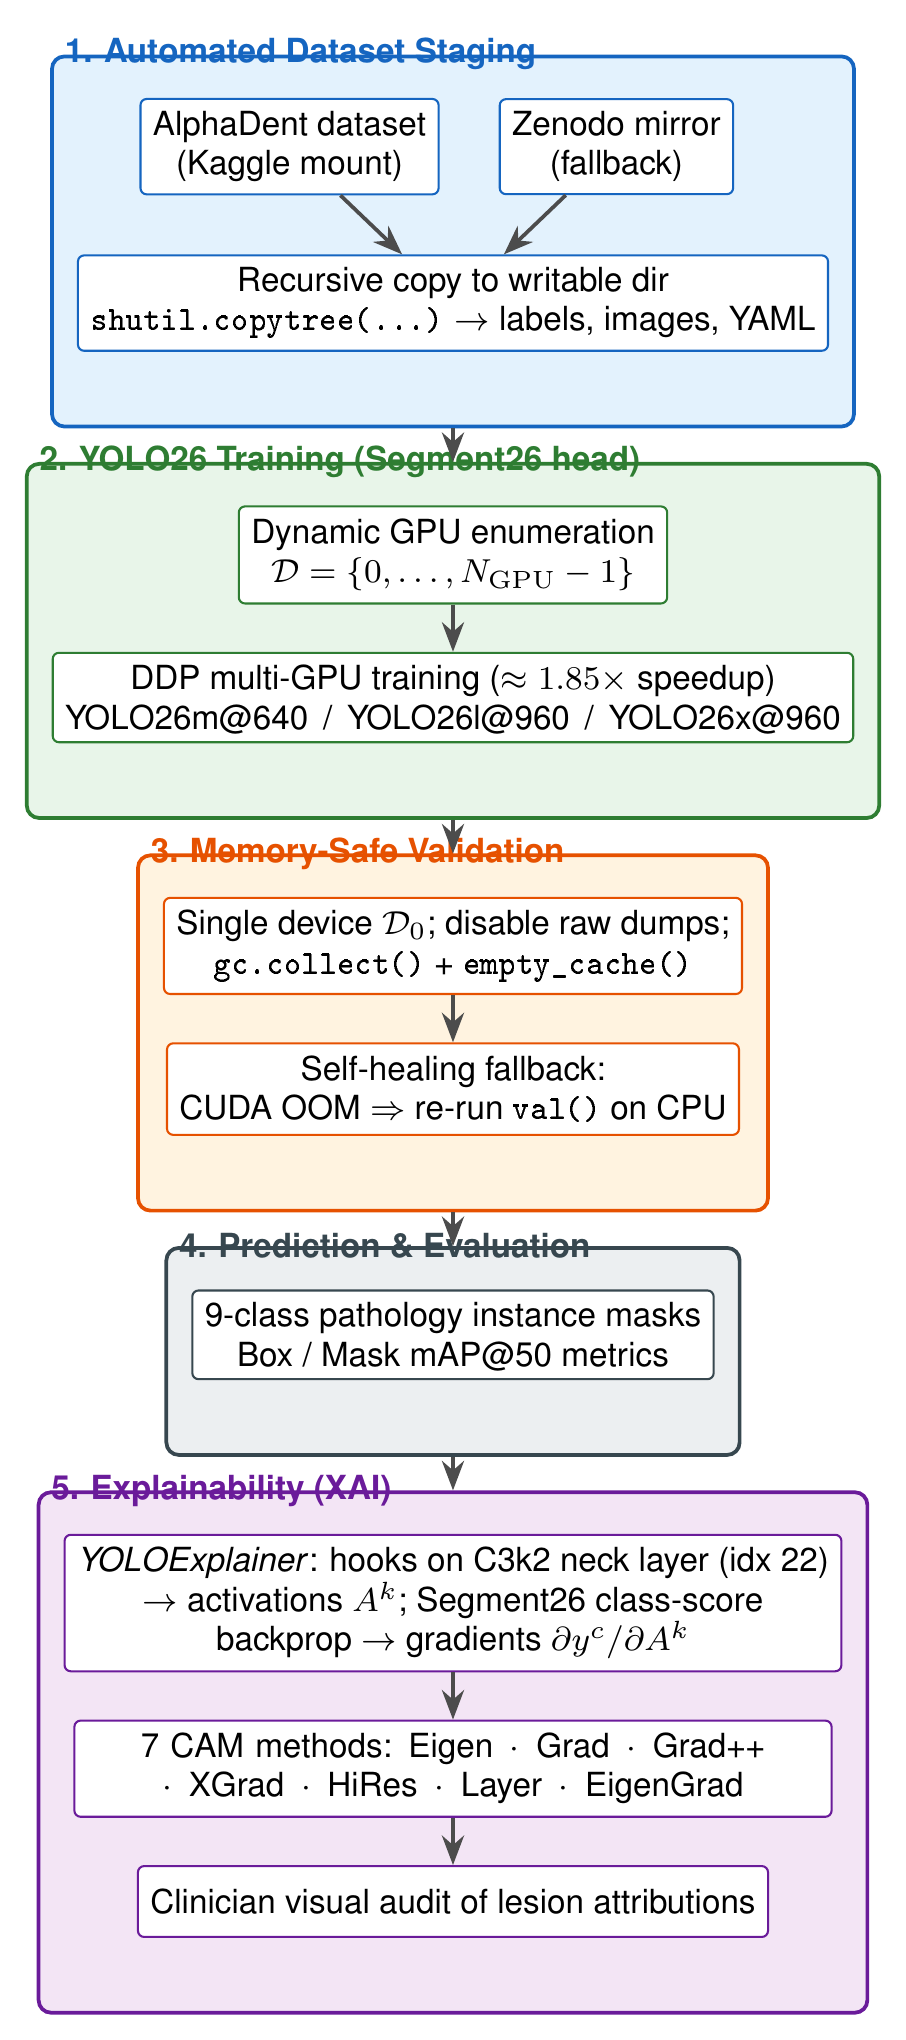
\includegraphics[width=\textwidth]{fig_pipeline.png}
\caption{Overview of the proposed interpretable YOLO26 pipeline for dental pathology instance segmentation: automated dataset staging, DDP multi-GPU training with the Segment26 head, self-healing memory-safe validation, prediction and evaluation, and multi-method explainability with a quantitative faithfulness/agreement assessment that identifies Eigen-CAM as the most faithful attribution.}
\label{fig:pipeline}
\end{figure*}

\subsection{Data Collection}
We use AlphaDent~\cite{sosnin2025alphadent}, a set of high-resolution intra-oral photographs annotated with polygon instance masks for nine dentist-defined pathology classes, caries among them. A small but instructive detail: symbolically linking the label directory from a read-only competition mount seems harmless, but YOLO writes \texttt{.cache} scan files next to the labels, so training crashes. The pipeline therefore copies images, labels, and the dataset YAML recursively into a writable working directory (\texttt{shutil.copytree(..., dirs\_exist\_ok=True)}), falling back to a Zenodo download when the competition mount is absent. We train at two input scales, 640$\times$640 (YOLO26m) and 960$\times$960 (YOLO26l, YOLO26x), matching the two baseline YOLOv8x resolutions.

\subsection{Analysis}
\subsubsection{YOLO26 Architecture}
YOLO26~\cite{jocher2026yolo26} is a unified, end-to-end real-time vision model family. We use its instance segmentation variants, whose \texttt{Segment26} head predicts prototype masks and per-instance coefficients in the YOLACT style~\cite{bolya2019yolact}, decoded jointly with box regression and nine-class logits. The size difference from the baseline is what makes chairside deployment plausible: YOLOv8x-seg carries 71.8M parameters and 344.1 GFLOPs, while YOLO26m-seg needs 23.5M parameters and 121.2 GFLOPs (fused), reductions of 67.2\% and 64.8\%.

\subsubsection{Dynamic Multi-GPU Training with DDP}
The baseline scripts hard-code \texttt{device=[0]}, so a second GPU sits idle unless the user edits the source. We instead enumerate whatever is available at runtime,
\begin{equation}
\mathcal{D} = \{0, 1, \dots, N_{\mathrm{GPU}}-1\},
\end{equation}
and launch DDP training across all of it. Validation and prediction are deliberately routed back to a single device ($\mathcal{D}_0$): DDP validation loops are prone to multi-threaded metric-aggregation conflicts, and a single device sidesteps them entirely. On two Tesla T4 GPUs, 50 epochs finish in 1.46 hours, roughly a 1.85$\times$ speedup over the single-GPU configuration.

\subsubsection{Self-Healing Memory-Safe Validation}
This component exists because validation kept crashing. AlphaDent images are very large, and with \texttt{save\_json} or \texttt{save\_txt} enabled, YOLO reconstructs masks at full resolution via bilinear interpolation; on multi-instance images this transiently allocates up to 15.69~GiB and kills the GPU kernel. A naive retreat to the CPU fails differently, since holding all the scaled float tensors in system RAM invites the OS OOM killer instead. The routine we settled on does three things: it disables raw-prediction dumping so metrics are computed on downscaled mask grids, it flushes memory (\texttt{gc.collect()}, \texttt{torch.cuda.empty\_cache()}) before evaluation, and it wraps the whole call in a fallback that catches CUDA OOM errors and re-runs on CPU, as summarized in Algorithm~\ref{alg:selfheal}.

\begin{algorithm}[htbp]
\caption{Self-Healing Memory-Safe Validation}
\label{alg:selfheal}
\begin{algorithmic}[1]
\STATE Disable \texttt{save\_json}, \texttt{save\_txt}, \texttt{save\_conf}
\STATE \texttt{gc.collect()}; \texttt{torch.cuda.empty\_cache()}
\STATE \textbf{try:} $\text{metrics} \leftarrow \texttt{model.val}(\text{device}=\mathcal{D}_0,\ \text{batch}=1,\ \text{FP16})$
\STATE \textbf{except} RuntimeError $e$:
\IF{``out of memory'' $\in$ $e$}
\STATE \texttt{gc.collect()}; \texttt{torch.cuda.empty\_cache()}
\STATE $\text{metrics} \leftarrow \texttt{model.val}(\text{device}=\text{CPU},\ \text{batch}=1,\ \text{FP32})$
\ELSE
\STATE \textbf{raise} $e$
\ENDIF
\end{algorithmic}
\end{algorithm}

We also fixed a quiet but severe bug in the baseline CLI: \texttt{--conf} and \texttt{--iou} were declared as \texttt{type=int}, which truncates a threshold like 0.001 to 0. All thresholds in our pipeline are plain, type-safe Python floats.

\subsubsection{Explainability: The YOLOExplainer Framework}
A prediction a clinician cannot inspect is a prediction they cannot trust, so we built explainability into the pipeline rather than bolting it on. \textit{YOLOExplainer} registers forward and backward hooks on a chosen intermediate YOLO26 layer, by default the final \texttt{C3k2} neck block (layer index 22), to capture feature activations $A^k$. It then back-propagates the summed per-class score from the \texttt{Segment26} head output to obtain gradients $\partial y^c / \partial A^k$, from which class activation maps are computed. If no target class is given, the module explains whichever of the nine pathology channels has the largest aggregate score. Generic CAM wrappers do not handle modern YOLO segmentation outputs; this one operates directly on \texttt{Segment26} predictions and supports seven attribution methods:

\begin{enumerate}
\item \textbf{Eigen-CAM}~\cite{muhammad2020eigen}: first principal component of the 2D activations; gradient-free and highly robust.
\item \textbf{Grad-CAM}~\cite{selvaraju2017grad}: activations weighted by spatially averaged class-score gradients.
\item \textbf{Grad-CAM++}~\cite{chattopadhay2018grad}: second-order gradient weighting, which helps when several lesions co-occur.
\item \textbf{XGrad-CAM}~\cite{fu2020axiom}: gradients scaled by normalized activations to satisfy sensitivity and conservation axioms.
\item \textbf{HiRes-CAM}~\cite{draelos2020use}: element-wise activation--gradient product, with a guarantee of faithfulness to the decision path.
\item \textbf{Layer-CAM}~\cite{jiang2021layercam}: positive-gradient spatial weighting of intermediate layers, useful for fine detail.
\item \textbf{EigenGrad-CAM}: first principal component of the gradient--activation product, pairing Eigen-CAM's robustness with class discrimination.
\end{enumerate}

Why seven methods instead of one? Because each has known failure modes, and showing them side by side (Fig.~\ref{fig:xai}) lets a clinician check whether the attributions agree before trusting any of them, which is much closer to how the causability literature says medical explanations should work~\cite{holzinger2019causability, borah2024comprehensive}.

\begin{figure}[htbp]
\centering
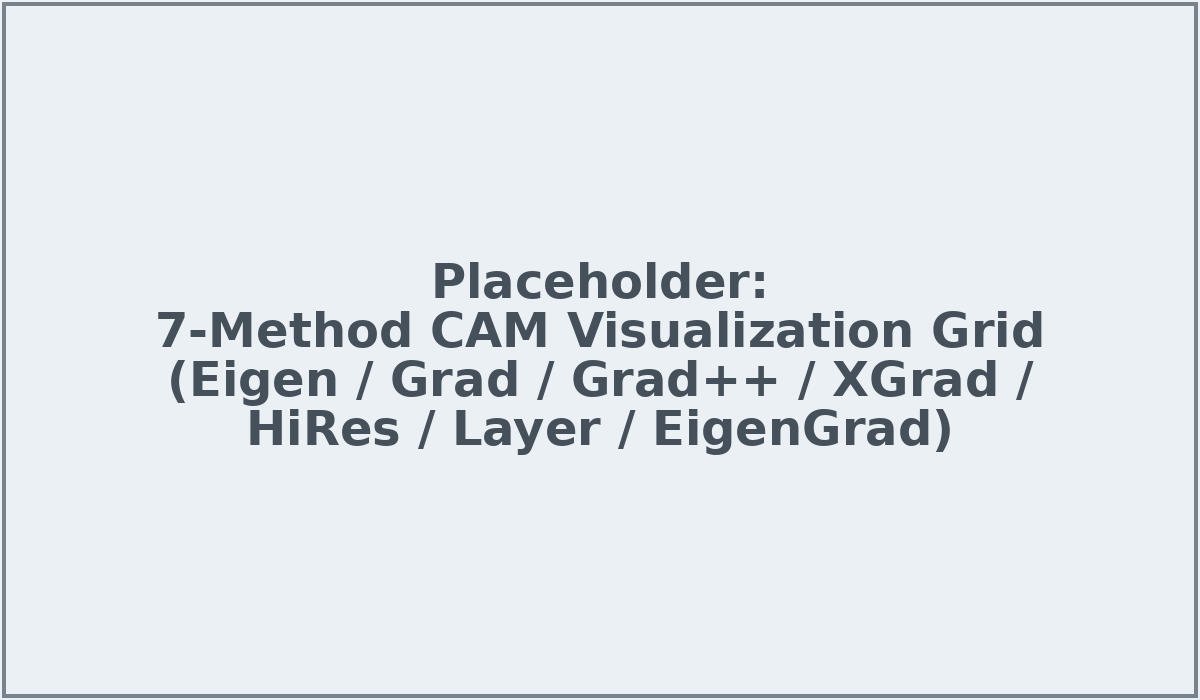
\includegraphics[width=0.48\textwidth]{fig_xai.png}
\caption{Class activation maps produced by the seven XAI methods for a caries instance predicted by YOLO26 on an AlphaDent intra-oral photograph.}
\label{fig:xai}
\end{figure}

\section{Results and Discussions}
\subsection{Experimental Setup}
All models are trained on AlphaDent with the Ultralytics framework for 100 epochs, using DDP across two Tesla T4 GPUs with default Ultralytics segmentation hyperparameters and augmentation; runs use batch size 16, falling back to 8 for YOLO26l and YOLO26x at 960 px under GPU memory limits. Validation runs at batch size 1 with FP16 inference on GPU (full precision on the CPU fallback), a confidence threshold of 0.001, and an IoU threshold of 0.5; for qualitative figures we raise the confidence threshold to 0.25 for visual clarity. The baseline YOLOv8x-seg is evaluated at 640 px and 960 px; our YOLO26m-seg and YOLO26l-seg are trained at both resolutions and YOLO26x-seg at 960 px. We report metrics at each run's best checkpoint (\texttt{best.pt}), selected by the framework's fitness criterion; this is the checkpoint that would actually be deployed. The baseline figures are the dataset authors' published all-class averages, computed with mask IoU~\cite{sosnin2025alphadent}, so baseline comparisons are made against our Mask mAP@50 column. Following the dataset authors' protocol~\cite{sosnin2025alphadent}, we additionally train YOLO26m and YOLO26l with the six caries classes merged into one (four classes in total). For the explainability evaluation we sample 30 validation images per configuration and score each of the seven CAMs with the causal deletion/insertion protocol (20 perturbation steps, trapezoidal AUC); inter-method agreement is the mean pairwise Spearman correlation between the seven heatmaps of a given image. Table~\ref{tab:complexity} compares model complexity, Table~\ref{tab:results} reports nine-class accuracy, Table~\ref{tab:results4} the merged-class results, and Table~\ref{tab:faith} the pooled XAI faithfulness. All accuracy numbers are from single training runs without confidence intervals or significance testing, and the XAI evaluation covers 30 validation images whose detected instances span four of the nine pathology classes; the reported margins should be read accordingly. Cells marked ``--'' correspond to baseline results not published in usable form by the reference pipeline.

\begin{table}[htbp]
\caption{Model Complexity Comparison}
\label{tab:complexity}
\centering
\begin{adjustbox}{max width=0.48\textwidth}
\begin{tabular}{lccc}
\toprule
\textbf{Model} & \textbf{Input (px)} & \textbf{Params (M)} & \textbf{GFLOPs} \\
\midrule
YOLOv8x-seg (baseline)~\cite{jocher2023ultralytics} & 640 / 960 & 71.8 & 344.1 \\
\rowcolor{highlightColor}
YOLO26m-seg (ours) & 640 / 960 & \textbf{23.5} & \textbf{121.2} \\
\rowcolor{highlightColor}
YOLO26l-seg (ours) & 640 / 960 & 27.9 & 139.4 \\
\rowcolor{highlightColor}
YOLO26x-seg (ours) & 960 & 62.7 & 313.0 \\
\midrule
\multicolumn{2}{l}{Reduction (26m vs.\ v8x)} & $-67.2\%$ & $-64.8\%$ \\
\bottomrule
\end{tabular}
\end{adjustbox}
\end{table}

\begin{table}[htbp]
\caption{Instance Segmentation Results on AlphaDent (Best Checkpoint, 100-Epoch Schedule)}
\label{tab:results}
\centering
\begin{adjustbox}{max width=0.48\textwidth}
\begin{tabular}{lccc}
\toprule
\textbf{Model} & \textbf{Input (px)} & \textbf{Box mAP@50} & \textbf{Mask mAP@50} \\
\midrule
YOLOv8x-seg (baseline)~\cite{sosnin2025alphadent} & 640 & -- & -- \\
YOLOv8x-seg (baseline)~\cite{sosnin2025alphadent} & 960 & -- & 0.436 \\
\rowcolor{highlightColor}
YOLO26m-seg (ours) & 640 & \textbf{0.4658} & 0.4455 \\
\rowcolor{highlightColor}
YOLO26m-seg (ours) & 960 & 0.4397 & 0.4316 \\
\rowcolor{highlightColor}
YOLO26l-seg (ours) & 640 & 0.4487 & 0.4327 \\
\rowcolor{highlightColor}
YOLO26l-seg (ours) & 960 & 0.4641 & \textbf{0.4582} \\
\rowcolor{highlightColor}
YOLO26x-seg (ours) & 960 & 0.4449 & 0.4292 \\
\bottomrule
\end{tabular}
\end{adjustbox}
\end{table}

\subsection{Accuracy--Efficiency Trade-off}
The headline result is that the smaller model does not merely approach the baseline, it beats it. The dataset authors report 0.436 mask-IoU mAP@50 for YOLOv8x-seg at 960 px~\cite{sosnin2025alphadent}. YOLO26m-seg at 640 px reaches 0.4455 Mask mAP@50 (0.4658 Box), exceeding the published baseline by 0.95 points while using about a third of the parameters and 35.2\% of the compute. For a screening tool that has to run on modest hardware, this is no longer a trade-off at all. At 960 px, YOLO26l-seg reaches the best Mask mAP@50 of the family, 0.4582 (0.4641 Box), 2.2 points above the published baseline, with 27.9M parameters and 139.4 GFLOPs, i.e.\ 61.1\% fewer parameters and 59.5\% less compute than YOLOv8x at the same resolution. The grid also reveals a capacity--resolution interaction: the medium model is strongest at 640 px (0.4658 vs.\ 0.4397 at 960 px), whereas the large model prefers 960 px (0.4641 vs.\ 0.4487 at 640 px). Scaling further does not help: YOLO26x-seg at 960 px lands at 0.4449/0.4292, below YOLO26l at the same resolution. On a dataset of AlphaDent's size, with several rare pathology classes, the largest model appears to overfit rather than benefit from added capacity, a pattern consistent with its higher validation precision but markedly lower recall. The pipeline also reports structured Mask mAP@50 benchmarks, which the baseline CLI never published in usable form and which matter for pixel-accurate lesion delineation. Qualitative predictions across the nine pathology classes are shown in Fig.~\ref{fig:preds}.

\begin{figure}[htbp]
\centering
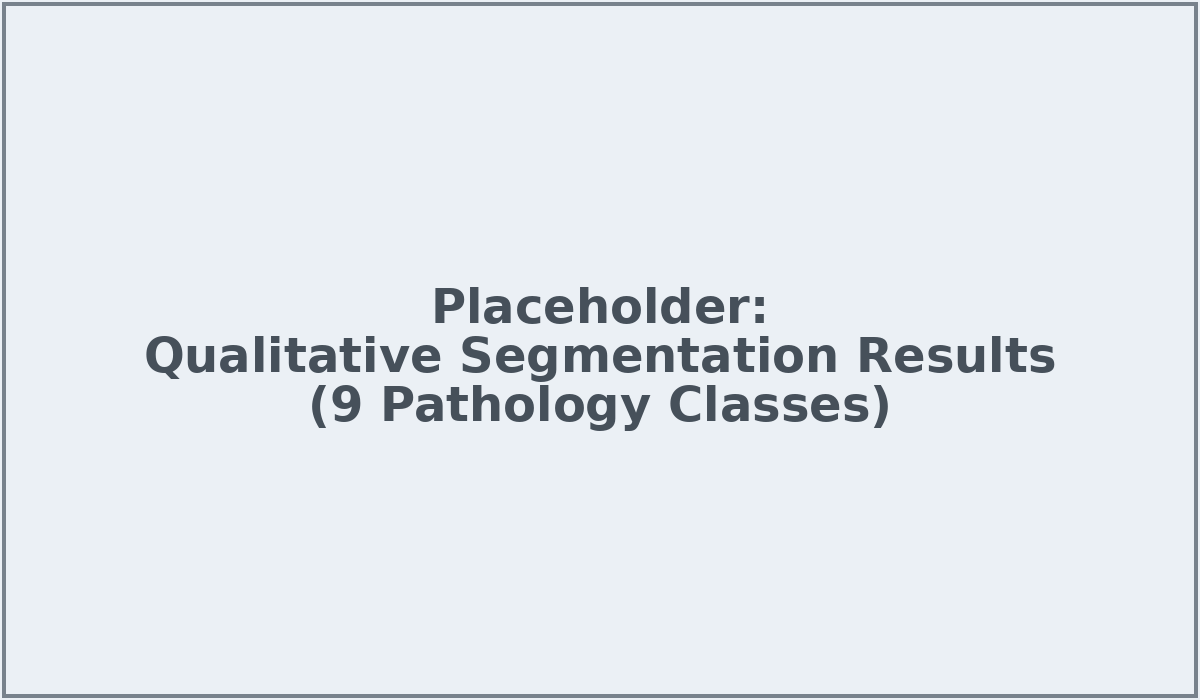
\includegraphics[width=0.48\textwidth]{fig_predictions.png}
\caption{Qualitative instance segmentation results of the proposed YOLO26 models on AlphaDent test images (nine pathology classes).}
\label{fig:preds}
\end{figure}

\subsection{Merged-Class (Four-Class) Results}
Several caries subclasses in AlphaDent are rare enough that per-class metrics are unstable, which is why the dataset authors also evaluate a merged protocol in which all six caries classes collapse into a single \textit{Caries} class~\cite{sosnin2025alphadent}. Table~\ref{tab:results4} reports our results under this protocol. YOLO26l-seg at 960 px reaches 0.6966 Box and 0.6913 Mask mAP@50, exceeding the published YOLOv8x baseline of 0.680, and it does so despite its schedule being truncated at 83 of 100 epochs by the compute budget, with metrics still improving at cutoff. Notably, the resolution preference seen in the nine-class setting inverts: with the coarser label space, both the medium and large models benefit from 960 px inputs (0.6934 vs.\ 0.6764 for YOLO26m; 0.6966 vs.\ 0.6739 for YOLO26l).

\begin{table}[htbp]
\caption{Merged Four-Class Results on AlphaDent (Best Checkpoint)}
\label{tab:results4}
\centering
\begin{adjustbox}{max width=0.48\textwidth}
\begin{tabular}{lccc}
\toprule
\textbf{Model} & \textbf{Input (px)} & \textbf{Box mAP@50} & \textbf{Mask mAP@50} \\
\midrule
YOLOv8x-seg (baseline)~\cite{sosnin2025alphadent} & 960 & -- & 0.680 \\
\rowcolor{highlightColor}
YOLO26m-seg (ours) & 640 & 0.6764 & 0.6729 \\
\rowcolor{highlightColor}
YOLO26m-seg (ours) & 960 & 0.6934 & 0.6772 \\
\rowcolor{highlightColor}
YOLO26l-seg (ours) & 640 & 0.6739 & 0.6740 \\
\rowcolor{highlightColor}
YOLO26l-seg (ours) & 960 & \textbf{0.6966} & \textbf{0.6913} \\
\bottomrule
\end{tabular}
\end{adjustbox}
\end{table}

\subsection{Training Scalability and Robustness}
DDP scaling behaved close to linearly in practice: 50 epochs on two T4 GPUs took 1.46 hours, about 1.85$\times$ faster than the single-GPU setup (a sub-linear 0.93 scaling efficiency on two GPUs). The memory-safe validation routine did the job it was built for. The transient 15.69~GiB allocations that used to abort high-resolution evaluation simply no longer occur, and on the rare occasion an OOM does slip through, the CPU fallback absorbs it and the run finishes rather than dies.

\subsection{Interpretability: Qualitative Observations}
Looking across the CAM methods, the attributions for correctly detected caries instances concentrate where a dentist would want them to: on the lesion surface and the adjacent enamel margins. Eigen-CAM, being gradient-free, stays the most stable under the specular reflections that plague intra-oral photography and yields the cleanest lesion-centred maps; the gradient-based methods, which as shown below coincide on this architecture, produce a single shared, noisier attribution pattern.

\subsection{Quantitative XAI Faithfulness}
We move beyond visual inspection with a causal faithfulness evaluation on 30 validation images per configuration. Pixels are progressively removed (deletion) or revealed (insertion) in CAM-importance order over 20 steps, and the resulting confidence curve is integrated: a faithful map yields a \emph{low} deletion AUC, because removing the pixels it deems salient collapses the prediction quickly, and a \emph{high} insertion AUC, because revealing them restores confidence quickly. Table~\ref{tab:faith} pools these AUCs per method across all five configurations. A notable architectural finding emerges: at the YOLO26 neck the class-score gradient is non-negative, so several gradient-based CAMs coincide \emph{exactly} --- HiRes-CAM equals Layer-CAM (Layer-CAM's positive-gradient clamp becomes a no-op) and Grad-CAM equals Grad-CAM++ --- collapsing the seven nominal methods into three distinct behaviours. Among them the gradient-free Eigen-CAM is the most faithful by a clear margin: the best insertion AUC (0.633), the lowest deletion AUC (0.497), and by far the largest insertion-minus-deletion margin ($+0.136$), against near-neutral margins ($\leq\!0.03$) for the gradient family. Fig.~\ref{fig:faith} shows the full per-method distributions. The result is clinically convenient: the method most robust to specular reflection is also the most faithful, making Eigen-CAM a sound default for a chairside audit view. With $n{=}30$ images the per-method AUC spread is wide, so differences \emph{within} the gradient family are not statistically separated.

\begin{table}[htbp]
\caption{Pooled XAI faithfulness on AlphaDent (mean $\pm$ std over 30 images $\times$ 5 configurations). At the YOLO26 neck the class gradient is non-negative, so several CAMs coincide \emph{exactly} (marked ``$\equiv$''); the seven nominal methods reduce to three distinct behaviours.}
\label{tab:faith}
\centering
\begin{adjustbox}{max width=0.48\textwidth}
\begin{tabular}{lccc}
\toprule
\textbf{Method} & \textbf{Deletion AUC}\,$\downarrow$ & \textbf{Insertion AUC}\,$\uparrow$ & \textbf{Ins.$-$Del.} \\
\midrule
\rowcolor{highlightColor}
Eigen-CAM (gradient-free) & \textbf{0.497} $\pm$ 0.378 & \textbf{0.633} $\pm$ 0.293 & $\mathbf{+0.136}$ \\
EigenGrad-CAM & 0.544 $\pm$ 0.144 & 0.557 $\pm$ 0.162 & $+0.013$ \\
HiRes-CAM $\equiv$ Layer-CAM & 0.533 $\pm$ 0.127 & 0.559 $\pm$ 0.133 & $+0.026$ \\
Grad-CAM $\equiv$ Grad-CAM++ & 0.543 $\pm$ 0.177 & 0.552 $\pm$ 0.165 & $+0.009$ \\
XGrad-CAM & 0.546 $\pm$ 0.173 & 0.551 $\pm$ 0.165 & $+0.005$ \\
\bottomrule
\end{tabular}
\end{adjustbox}
\end{table}

\begin{figure}[htbp]
\centering
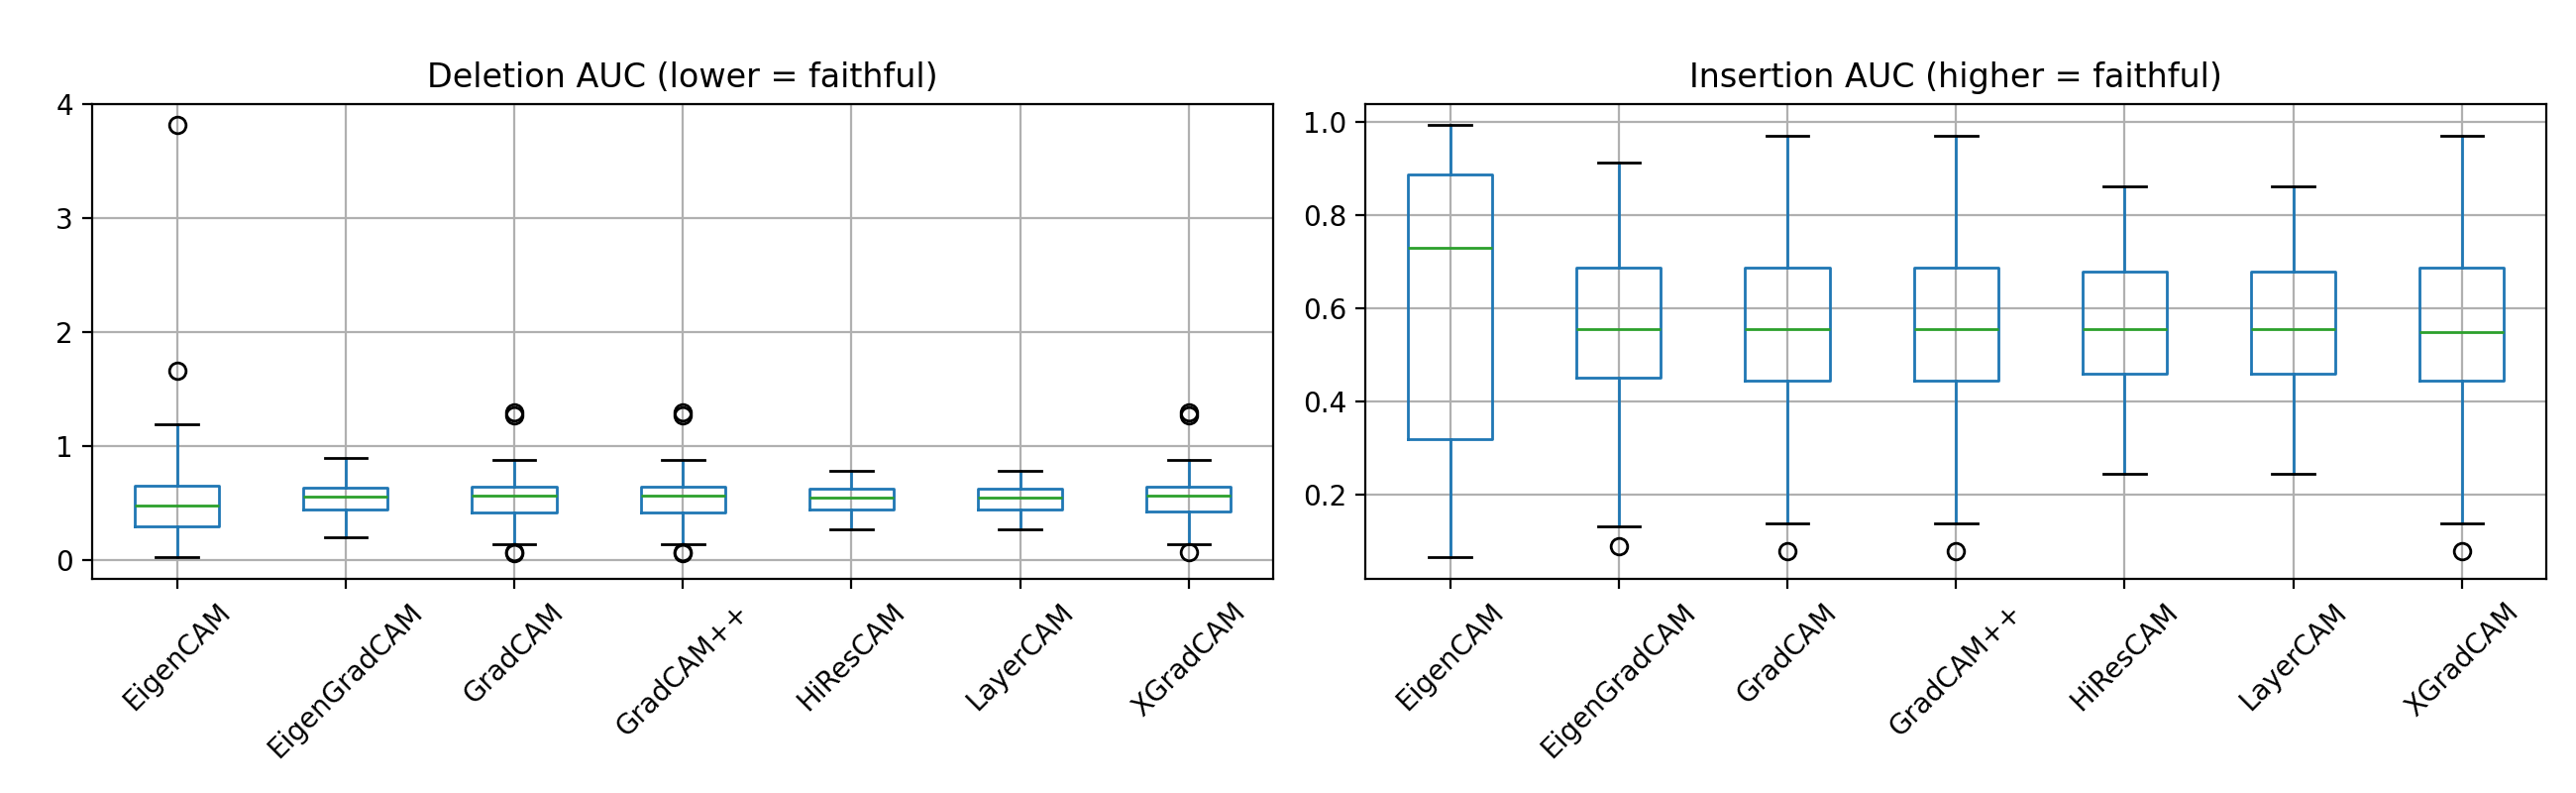
\includegraphics[width=0.48\textwidth]{fig_faithfulness.png}
\caption{Per-method causal faithfulness across all configurations: deletion AUC (lower is more faithful) and insertion AUC (higher is more faithful). Eigen-CAM leads on both.}
\label{fig:faith}
\end{figure}

\subsection{Inter-Method Agreement}
We also quantify how much the seven maps agree, per image, as the mean pairwise Spearman correlation between them. Because the gradient-based maps coincide while Eigen-CAM is markedly different, cross-method agreement is low overall (mean $\approx 0.05$ across the 150 image--configuration pairs). Importantly, and contrary to an intuitive assumption, agreement does \emph{not} track prediction correctness: it is essentially identical for correct and incorrect predictions ($0.053$ vs.\ $0.049$; Mann--Whitney $p=0.24$) and is uncorrelated with model confidence (Spearman $=0.11$), as Fig.~\ref{fig:agree} shows. Agreement is therefore a descriptive summary of attribution stability but, on this dataset, should not be read as a confidence signal on its own~\cite{adadi2018peeking}, a caution worth stating explicitly before clinical deployment.

\begin{figure}[htbp]
\centering
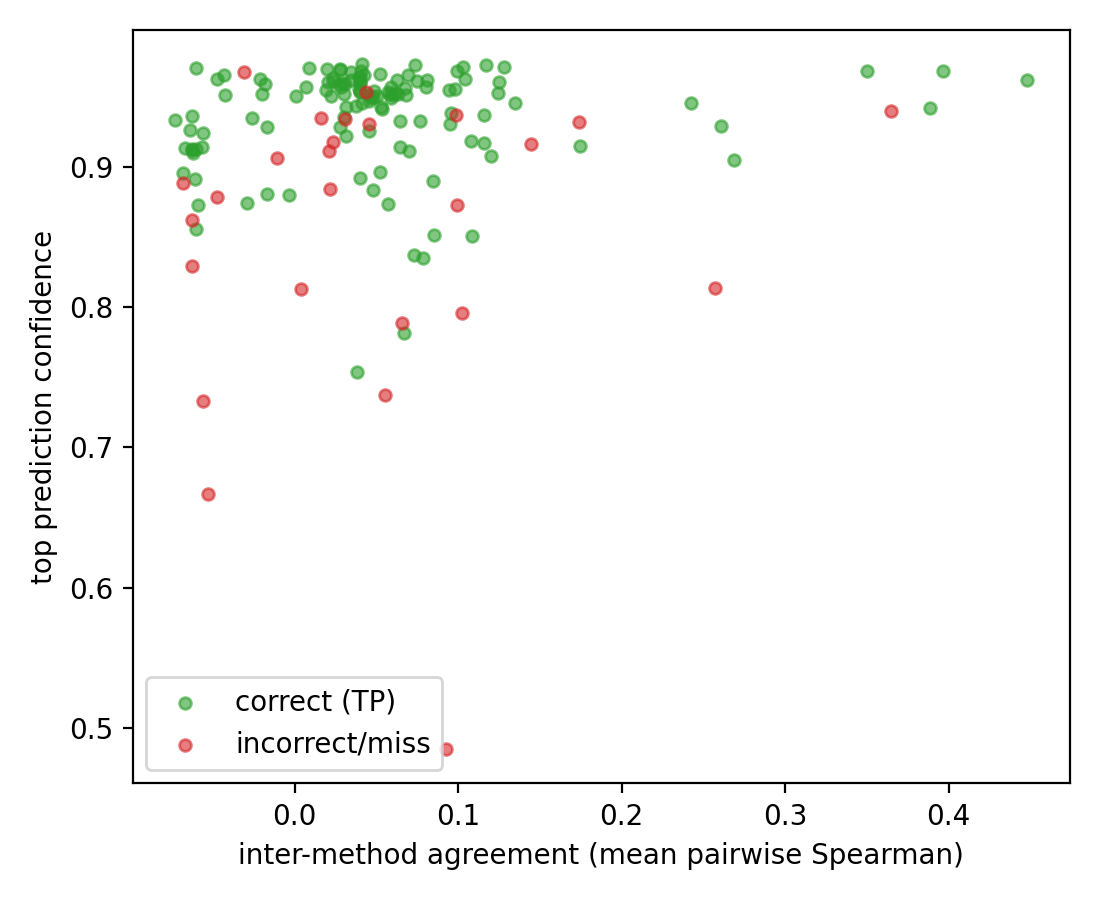
\includegraphics[width=0.42\textwidth]{fig_agreement.png}
\caption{Inter-method agreement (mean pairwise Spearman across the seven CAMs) versus top prediction confidence, coloured by correctness. Correct and incorrect predictions overlap across the full agreement range, so agreement alone does not indicate reliability.}
\label{fig:agree}
\end{figure}

\section{Discussion}
The main takeaway is that shrinking from a 71.8M-parameter YOLOv8x to a 23.5M-parameter YOLO26m costs nothing on this task: at its best checkpoint the smaller model is 0.95 Mask mAP@50 points above the published baseline, at a 64.8\% compute saving, which makes chairside and mobile deployment realistic without server-class hardware. It is worth being honest about what the engineering contributions are: DDP orchestration, automated dataset staging, type-safe thresholds, and OOM-resilient validation do not make the model smarter, but they remove exactly the kind of reproducibility failures that stall clinical ML pipelines in practice. A second takeaway is that capacity must match data and resolution: YOLO26l exceeds the baseline at 960 px by a wider margin (0.4582 vs.\ 0.436 Mask mAP@50) but weakens at 640 px, YOLO26m shows the opposite preference, and the extra-large YOLO26x underperforms both, suggesting that on a single moderately sized clinical dataset the biggest model is the wrong choice, not just the most expensive one. Limitations remain. Evaluation is on a single dataset and the 640 px baseline run is not published; and while we now quantify attribution faithfulness with deletion/insertion curves and inter-method agreement, this rests on 30 validation images per configuration, and the reported mAP differences are single-run and not significance-tested, so both larger-scale evaluation and reader studies with practicing dentists remain the obvious next steps.

\section{Conclusion}
We set out to build a caries detector a clinic could actually run and a clinician could actually question, and the pieces are now in place: a YOLO26 pipeline that exceeds the published baseline (0.4455 vs.\ 0.436 Mask mAP@50) at a third of the size, near-linear multi-GPU training via DDP, validation that heals itself instead of crashing, and a seven-method CAM framework, quantitatively benchmarked for causal faithfulness, wired to the YOLO26 segmentation outputs. Across the family, YOLO26l at 960 px delivers the best masks (0.4582 Mask mAP@50) while YOLO26x overfits, confirming that model scale should be chosen against dataset size rather than maximized. Under the merged four-class protocol, YOLO26l surpasses the published baseline (0.6913 vs.\ 0.680 Mask mAP@50) at 61\% fewer parameters. Future work will extend evaluation to external intra-oral and radiographic datasets~\cite{uribe2024public} and put the explanations in front of dentists to measure their clinical value, building on the Eigen-CAM faithfulness ranking established here.

\bibliographystyle{IEEEtran}
\bibliography{Ref}
\end{document}
